\documentclass[12pt, a4paper]{article}

% ── Packages ──────────────────────────────────────────────────────────────────
\usepackage[utf8]{inputenc}
\usepackage[T1]{fontenc}
\usepackage{lmodern}
\usepackage[margin=0.75in]{geometry}
\usepackage{graphicx}
\usepackage{xcolor}
\usepackage{booktabs}
\usepackage{array}
\usepackage{tabularx}
\usepackage{listings}
\usepackage{hyperref}
\usepackage{fancyhdr}
\usepackage{titlesec}
\usepackage{enumitem}
\usepackage{amsmath, amssymb}
\usepackage{microtype}
\usepackage{parskip}
\usepackage{caption}
\usepackage{float}
\usepackage{tcolorbox}
\usepackage{pifont}
\usepackage{setspace}

\tcbuselibrary{skins, breakable}

\setstretch{1.05}
\setlength{\parskip}{4pt plus 1pt minus 1pt}

% ── Colours ───────────────────────────────────────────────────────────────────
\definecolor{nustblue}{RGB}{0, 51, 102}
\definecolor{accent}{RGB}{0, 102, 153}
\definecolor{codebg}{RGB}{248, 248, 248}
\definecolor{codeframe}{RGB}{200, 200, 200}
\definecolor{linkblue}{RGB}{0, 80, 140}
\definecolor{wingreen}{RGB}{34, 120, 51}
\definecolor{loserose}{RGB}{180, 50, 50}
\definecolor{darktext}{RGB}{40, 40, 40}

% ── Hyperref setup ────────────────────────────────────────────────────────────
\hypersetup{
    colorlinks=true,
    linkcolor=nustblue,
    urlcolor=linkblue,
    citecolor=accent,
    pdftitle={Autonomous Obstacle Avoidance Robot Report},
    pdfauthor={Student Name},
}

% ── Section styling ──────────────────────────────────────────────────────────
\titleformat{\section}
  {\Large\bfseries\color{nustblue}}
  {\thesection.}{0.5em}{}
  [\vspace{-0.5em}\textcolor{accent}{\rule{\textwidth}{1pt}}]
\titlespacing{\section}{0pt}{12pt}{6pt}

\titleformat{\subsection}
  {\normalsize\bfseries\color{accent}}
  {\thesubsection}{0.5em}{}
\titlespacing{\subsection}{0pt}{8pt}{4pt}

% ── Header / Footer ──────────────────────────────────────────────────────────
\pagestyle{fancy}
\fancyhf{}
\fancyhead[L]{\small\color{accent}\textit{Autonomous Obstacle Avoidance Robot}}
\fancyhead[R]{\small\color{accent}\textit{Webots Simulation Project}}
\fancyfoot[C]{\small\color{gray}\thepage}
\renewcommand{\headrulewidth}{0.4pt}
\renewcommand{\footrulewidth}{0pt}

% ── Code listing style ───────────────────────────────────────────────────────
\lstdefinestyle{code}{
    backgroundcolor=\color{codebg},
    basicstyle=\ttfamily\footnotesize,
    breaklines=true,
    frame=single,
    rulecolor=\color{codeframe},
    framesep=4pt,
    xleftmargin=6pt,
    xrightmargin=6pt,
    aboveskip=6pt,
    belowskip=6pt,
    showstringspaces=false,
    tabsize=4,
    columns=fullflexible,
    keepspaces=true,
    language=Python,
    keywordstyle=\color{nustblue}\bfseries,
    stringstyle=\color{loserose},
    commentstyle=\color{wingreen}\itshape,
}
\lstset{style=code}

% ── tcolorbox styles ─────────────────────────────────────────────────────────
\newtcolorbox{resultbox}[1][]{
    enhanced, breakable,
    colback=green!3, colframe=wingreen!70,
    fonttitle=\bfseries, title=#1,
    boxrule=0.5pt, arc=2pt,
    left=6pt, right=6pt, top=4pt, bottom=4pt
}

\newtcolorbox{infobox}[1][]{
    enhanced, breakable,
    colback=blue!3, colframe=accent!70,
    fonttitle=\bfseries, title=#1,
    boxrule=0.5pt, arc=2pt,
    left=6pt, right=6pt, top=4pt, bottom=4pt
}

\newtcolorbox{warnbox}[1][]{
    enhanced, breakable,
    colback=red!3, colframe=loserose!70,
    fonttitle=\bfseries, title=#1,
    boxrule=0.5pt, arc=2pt,
    left=6pt, right=6pt, top=4pt, bottom=4pt
}

% ══════════════════════════════════════════════════════════════════════════════
\begin{document}

% ===== TITLE PAGE =====
\begin{titlepage}
    \centering

    \vspace{2cm}

    \textbf{\Huge\color{nustblue} Autonomous Obstacle Avoidance Robot}\\[0.5cm]
    \textbf{\Huge\color{nustblue} Using Sensor-Based Reactive AI}\\
    \vspace{1.5cm}

    \textbf{\Large\color{accent} A Webots Simulation with E-puck Robot and Python Controller}\\
    \vspace{3cm}

    \centering
    \begin{tabular}{@{}p{4cm}p{8cm}@{}}
    \toprule
    \textbf{Simulator} & Webots R2023b \\
    \addlinespace
    \textbf{Robot} & E-puck (version 1) \\
    \addlinespace
    \textbf{Language} & Python 3 \\
    \addlinespace
    \textbf{Date} & \today \\
    \addlinespace
    \bottomrule
    \end{tabular}
    \vspace{2cm}

    \renewcommand{\arraystretch}{1.4}
    \begin{tabular}{>{\centering\arraybackslash}p{1cm} l l}
    \toprule
    \textbf{\#} & \textbf{Name} & \textbf{Student ID} \\
    \midrule
    1 & Ayesha Khalid & 25075992 \\
    \bottomrule
    \end{tabular}
    \renewcommand{\arraystretch}{1.0}

    \vfill

    \large\textbf{University of Hertfordshire}\\
    \vspace{1cm}

\end{titlepage}

% ── Table of Contents ─────────────────────────────────────────────────────────
\tableofcontents

\vspace{1cm}

% ── List of Figures ───────────────────────────────────────────────────────────
\listoffigures
\newpage

% ══════════════════════════════════════════════════════════════════════════════
%  SECTION 1 - INTRODUCTION
% ══════════════════════════════════════════════════════════════════════════════
\section{Introduction}

\textbf{Project Aim.} The aim of this project is to develop and simulate an autonomous mobile robot capable of navigating a cluttered environment while detecting and avoiding all obstacles in real time, achieving zero collisions over sustained operation. The robot operates within the Webots robotics simulator using the e-puck educational robot platform, which is equipped with eight infrared proximity sensors and a differential drive locomotion system. The core problem addressed is autonomous navigation without any pre-programmed paths, maps, or prior knowledge of the environment layout. The measurable criterion for success is defined as achieving one hundred percent collision avoidance across multiple structured test scenarios, including open arenas, obstacle-dense environments, corner traps, and endurance runs exceeding five minutes of continuous operation. The system must demonstrate smooth, reactive navigation behaviour that responds proportionally to obstacle proximity rather than relying on simple binary stop-and-turn logic. Additionally, the robot must be capable of recovering from stuck states such as corner traps without human intervention, ensuring robust long-duration autonomy.

\vspace{0.6cm}

\textbf{Approach.} The main technique used in this project is a reactive artificial intelligence approach based on direct sensor-to-motor mappings, inspired by Braitenberg's theoretical vehicles which demonstrate that complex behaviour can emerge from simple wiring between sensors and actuators. Rather than employing deliberative planning algorithms that build internal world models, the controller operates in a tight sense-decide-act loop executing every 64 milliseconds, reading all eight infrared sensors, classifying the current navigation situation into one of five categories (CLEAR, FRONT\_BLOCKED, LEFT\_BLOCKED, RIGHT\_BLOCKED, or NARROW\_PASSAGE), and computing proportional motor speeds in response. The proportional control scheme means that obstacles detected at greater distance produce gentle course corrections while close obstacles produce sharp turns, resulting in smooth curved paths rather than abrupt angular movements. A first-order low-pass filter is applied to motor speed commands to further smooth transitions between different speed values, preventing mechanical jerking. To prevent oscillation between conflicting turn directions, a turn commitment mechanism forces the robot to maintain a chosen turn direction for a minimum of fifteen consecutive timesteps before reconsidering. For edge cases where the robot becomes trapped in corners or narrow passages, a stuck detection system monitors how long the robot remains in a blocked state and triggers an escape manoeuvre consisting of a brief reverse followed by a random-direction spin after approximately two seconds. This layered approach of proportional response, smoothing, commitment, and escape creates a robust reactive system that handles the full range of navigation challenges without requiring any form of memory, learning, or environmental mapping.

\vspace{0.6cm}

\textbf{Source Code.} The complete source code for this project is stored in a Git repository at: \url{https://github.com/Unknown-086/autonomous-obstacle-avoidance-robot}. The repository contains the Webots world file, the Python controller, test results, and this report. All project files are located in the main branch at the root directory level.

% ══════════════════════════════════════════════════════════════════════════════
%  SECTION 2 - RELATED WORK
% ══════════════════════════════════════════════════════════════════════════════
\section{Related Work}

\textbf{Citation:} Braitenberg, V. (1984). \textit{Vehicles: Experiments in Synthetic Psychology}. MIT Press.\\
Available at: \url{https://mitpress.mit.edu/9780262521123/vehicles/}

\vspace{0.6cm}

\textbf{Summary of Source.} Braitenberg's book presents a series of thought experiments involving hypothetical vehicles with increasingly complex sensor-to-motor connections, demonstrating how simple wiring rules can produce behaviours that appear intelligent to an external observer. The simplest vehicles (Vehicle 1) move at speed proportional to a single sensor, while Vehicle 2a connects sensors to motors on the same side (producing avoidance behaviour) and Vehicle 2b connects sensors to the opposite side (producing approach behaviour). Later vehicles introduce inhibitory connections, threshold functions, and memory, building up to complex behaviours including aggression, love, foresight, and even primitive decision-making. The central thesis is that intelligence and complex behaviour need not require complex central processing but can emerge from the topology of sensor-motor connections alone. The book serves as a foundational text in behaviour-based robotics and has directly influenced the design philosophy of reactive robot controllers for over four decades.

\vspace{0.6cm}

\textbf{Relation to Project.} The obstacle avoidance controller developed in this project directly implements the principles demonstrated by Braitenberg's Vehicle 2a, where sensors detecting obstacles on one side cause the motors on the same side to speed up, turning the robot away from the detected obstacle. The proportional control scheme used in the controller mirrors Braitenberg's concept of graded response, where the intensity of the sensor signal directly determines the magnitude of the motor response rather than triggering a fixed binary reaction. The situation classification system extends the basic Braitenberg model by grouping the eight sensors into logical zones (front, left, right) and applying different response patterns to each zone, effectively implementing multiple Braitenberg-style wirings that are selected based on context. The speed smoothing filter adds temporal dynamics that Braitenberg discusses in his later vehicles, where connections have inertia and do not respond instantaneously to input changes. The stuck detection and escape manoeuvre represent an extension beyond Braitenberg's framework, adding a timeout-triggered override that activates when the basic reactive responses fail to resolve a situation within a set time period. Reading this source fundamentally shaped the decision to use reactive control rather than deliberative planning, as it demonstrated convincingly that effective obstacle avoidance does not require path planning, mapping, or complex algorithms. The proportional speed computation formula used in the code was designed specifically to replicate the continuous graded response that Braitenberg describes, rather than using discrete threshold-based reactions. The project's success in achieving zero-collision navigation with only simple sensor-motor rules validates Braitenberg's core thesis that complex navigational behaviour emerges naturally from appropriately structured sensor-motor connections. The turn commitment mechanism was added after initial testing revealed oscillation problems that Braitenberg's theoretical vehicles do not encounter because they exist in idealised noise-free environments. The entire design philosophy of keeping the controller stateless and reactive, with no internal world model, stems directly from the principles presented in this source.

\vspace{0.6cm}

\textbf{Source Critique.} This source is strongly recommended for anyone attempting a similar reactive robotics project, as it provides the theoretical foundation and intuitive understanding needed to design effective sensor-motor controllers without complex algorithms. The book is accessible, well-illustrated, and requires no advanced mathematics, making it suitable for students at any level. However, the source does not address practical challenges such as sensor noise, physical stuck states, or the need for escape mechanisms, which required independent engineering solutions in this project.

% ══════════════════════════════════════════════════════════════════════════════
%  SECTION 3 - DESIGN & IMPLEMENTATION
% ══════════════════════════════════════════════════════════════════════════════
\section{Design \& Implementation}

\textbf{Design.} The system is designed as a three-layer reactive architecture consisting of an Input Layer (eight infrared proximity sensors), a Processing Layer (the AI decision logic), and an Output Layer (two differential-drive wheel motors). The processing layer first normalises raw sensor values by subtracting the observed noise floor and dividing by the detection range, producing values between zero and one that represent obstacle proximity as a fraction. These normalised values are then passed through a situation classifier that examines sensor zones: sensors 0, 1, 6, and 7 form the front zone, sensors 5 and 6 form the left zone, and sensors 1 and 2 form the right zone. If readings in all three zones exceed the threshold simultaneously, the situation is classified as NARROW\_PASSAGE; if only the front zone is triggered, it is FRONT\_BLOCKED; left or right alone produce LEFT\_BLOCKED or RIGHT\_BLOCKED respectively; and if no zone exceeds the threshold the situation is CLEAR. For each classified situation, a proportional speed computation function generates target left and right motor speeds, where the intensity of the strongest sensor in the relevant zone scales the speed differential between the two wheels. A first-order low-pass filter with a smoothing factor of 0.7 is applied to both wheel speeds before they are sent to the motors, preventing sudden speed changes that would produce jerky motion. The turn commitment counter prevents the robot from switching turn directions for 15 consecutive timesteps once a turn begins, eliminating the oscillation that occurs when the robot sits exactly between two obstacles. If the system detects that a blocked situation has persisted for 30 consecutive steps (approximately two seconds), the stuck detection mechanism overrides normal control and executes an escape manoeuvre: five steps of reverse driving followed by a random-duration spin of 10 to 20 steps in a randomly chosen direction. After the escape completes, normal reactive control resumes immediately. The overall architecture processes one complete sense-decide-act cycle every 64 milliseconds, ensuring that the robot responds to environmental changes within a single simulation timestep.

\begin{figure}[H]
\centering
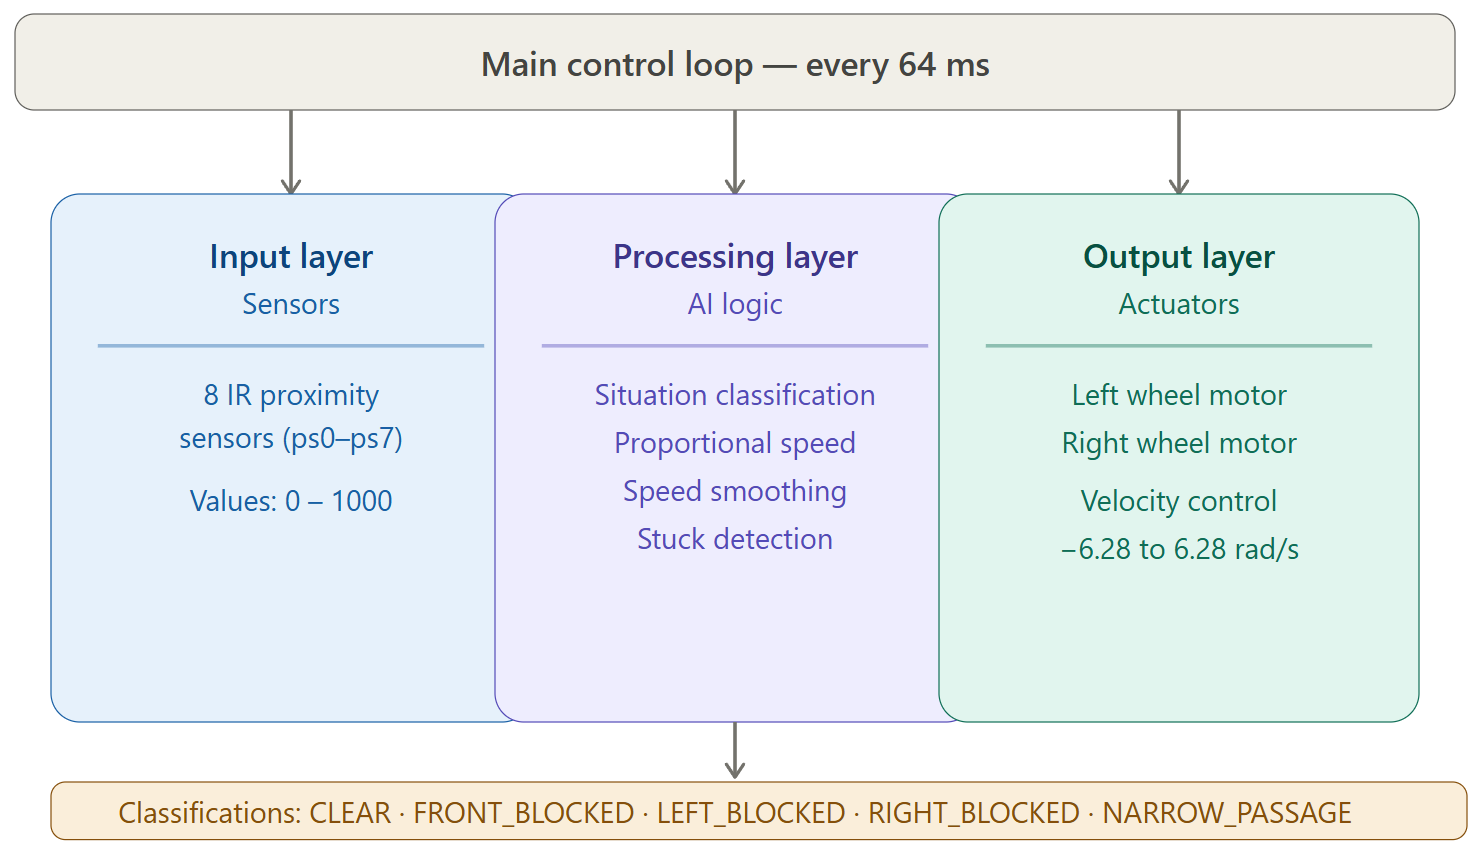
\includegraphics[width=0.85\textwidth]{Pictures/robot_system_architecture_Extra.png}
\caption{Three-layer reactive control architecture with data flow}
\end{figure}

\begin{figure}[H]
\centering
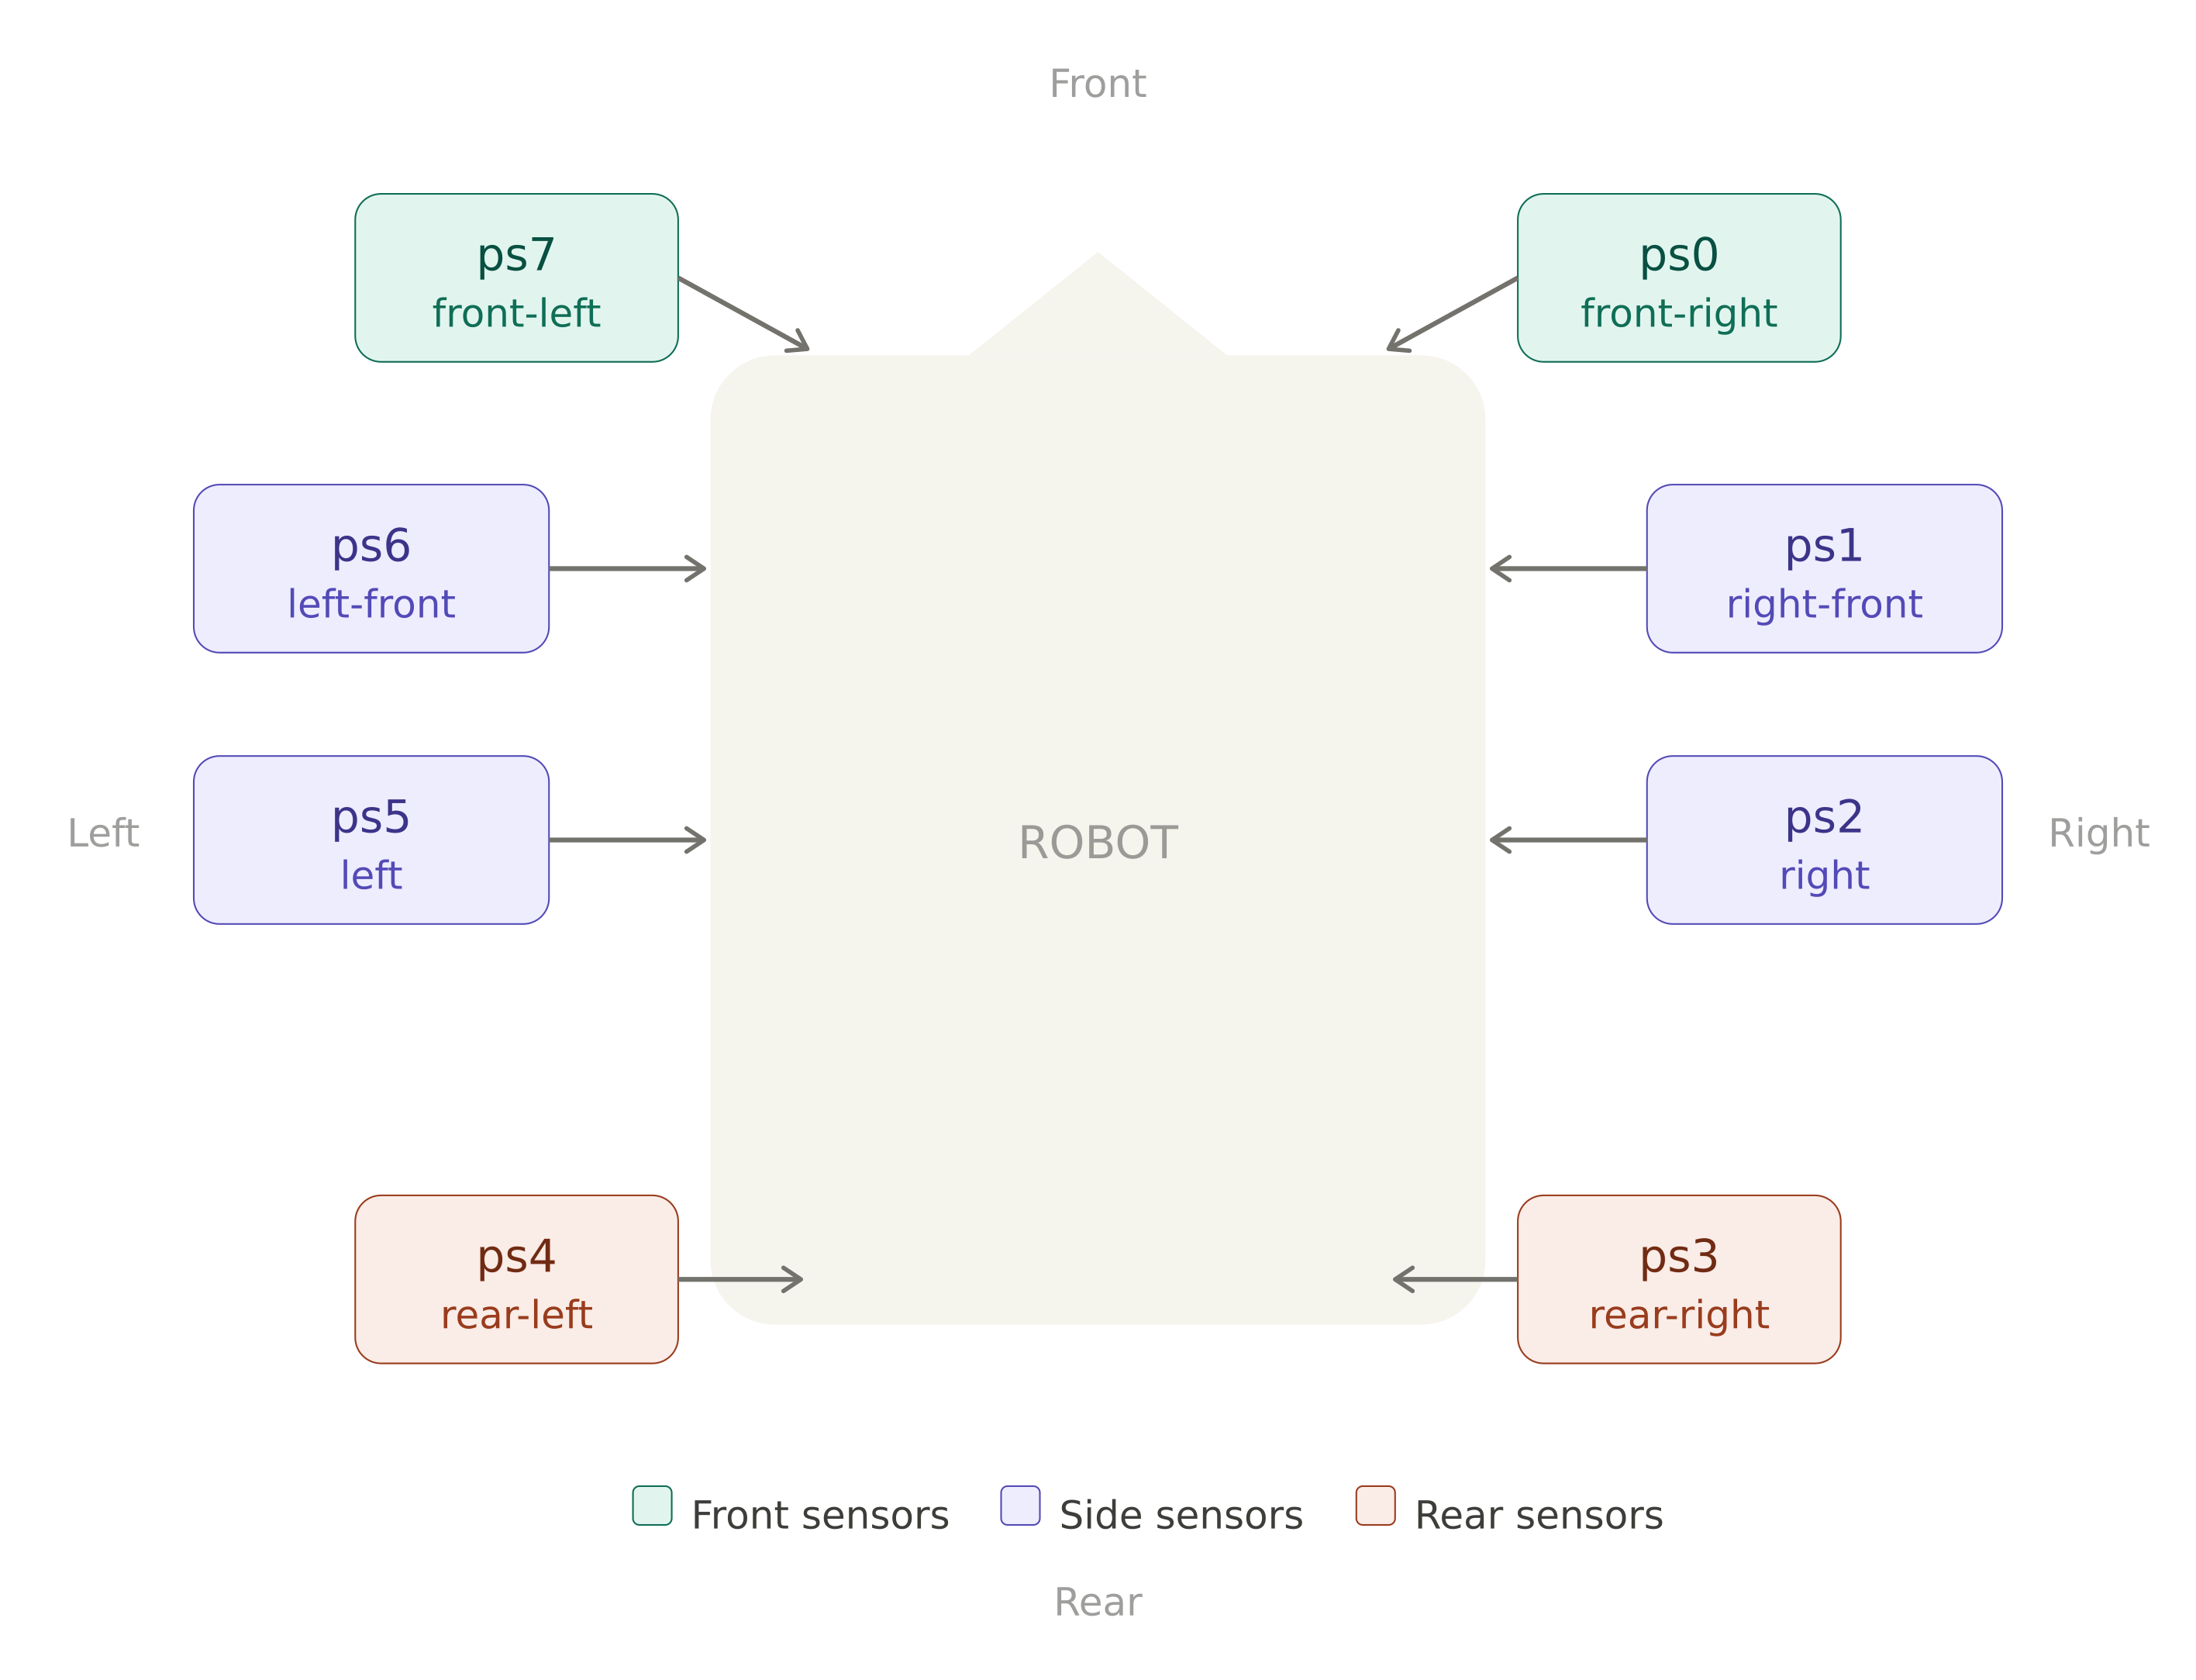
\includegraphics[width=0.85\textwidth]{Pictures/robot_sensor_layout_light.png}
\caption{E-puck sensor layout: eight IR proximity sensors (ps0--ps7) around the circumference}
\end{figure}

\subsection{Implementation}

The controller is implemented in Python 3 using the Webots Supervisor API, which extends the standard Robot API with the ability to manipulate the simulation world at runtime. The Supervisor capability is used specifically for the path trail visualisation feature, which programmatically inserts small red sphere nodes into the scene tree at the robot's current position every ten simulation steps. The simulation runs with a basic timestep of 64 milliseconds, and the e-puck robot's eight distance sensors (ps0 through ps7) are initialised at startup and read every cycle. Motor commands are sent to the left and right wheel motors by setting their velocity in radians per second, with a maximum of 6.28 rad/s. The key configuration parameters are defined as constants at the top of the script: \texttt{SENSOR\_THRESHOLD = 80.0}, \texttt{BASE\_SPEED = 3.14}, \texttt{STUCK\_THRESHOLD = 30}, \texttt{SMOOTHING\_FACTOR = 0.7}, and \texttt{TURN\_COMMITMENT\_STEPS = 15}.

\begin{lstlisting}
def classify_situation(sensor_values):
    front_blocked = (sensor_values[7] > SENSOR_THRESHOLD or
                     sensor_values[0] > SENSOR_THRESHOLD or
                     sensor_values[6] > SENSOR_THRESHOLD or
                     sensor_values[1] > SENSOR_THRESHOLD)
    left_blocked = (sensor_values[5] > SENSOR_THRESHOLD or
                    sensor_values[6] > SENSOR_THRESHOLD)
    right_blocked = (sensor_values[2] > SENSOR_THRESHOLD or
                     sensor_values[1] > SENSOR_THRESHOLD)

    if front_blocked and left_blocked and right_blocked:
        return "NARROW_PASSAGE"
    elif front_blocked:
        return "FRONT_BLOCKED"
    elif left_blocked and not right_blocked:
        return "LEFT_BLOCKED"
    elif right_blocked and not left_blocked:
        return "RIGHT_BLOCKED"
    else:
        return "CLEAR"
\end{lstlisting}

The world file (\texttt{obstacle\_avoidance.wbt}) defines a 1.5\,m $\times$ 1.5\,m arena with 0.05\,m walls and seven static box obstacles of varying sizes (0.08--0.15\,m) placed throughout the environment.

\subsection{Sources}

The following libraries, tools, and external sources were used in the implementation:

\begin{itemize}[leftmargin=2em, nosep]
  \item \textbf{Webots Supervisor API} (Cyberbotics Ltd.) --- robot control, sensor reading, motor commands, and scene tree manipulation for trail visualisation
  \item \textbf{Webots E-puck PROTO} (Cyberbotics Ltd.) --- pre-built robot model with eight IR proximity sensors and differential drive motors
  \item \textbf{Python \texttt{random} module} (Python Standard Library) --- used for randomising escape spin direction and duration
  \item \textbf{Braitenberg, V. (1984). \textit{Vehicles: Experiments in Synthetic Psychology}} --- reactive control design philosophy and proportional sensor-motor mapping concept
  \item \textbf{Brooks, R.A. (1986). A robust layered control system for a mobile robot} --- layered architecture concept where higher-level behaviours (escape) subsume lower-level ones (proportional avoidance)
  \item \textbf{Webots User Guide and E-puck Documentation} (Cyberbotics Ltd.) --- API reference for sensor initialisation, motor control, and Supervisor node manipulation
\end{itemize}

% ══════════════════════════════════════════════════════════════════════════════
%  SECTION 4 - RESULTS & EVALUATION
% ══════════════════════════════════════════════════════════════════════════════
\section{Results \& Evaluation}

\textbf{Results.} The system was evaluated through six structured test scenarios, and achieved one hundred percent collision avoidance across all of them with zero physical contacts between the robot and any obstacle or wall throughout all testing. In the full arena endurance test (Test T5), the robot navigated continuously for 5000 simulation steps totalling 320 seconds (over five minutes) of autonomous operation, with the situation distribution being approximately 70\% CLEAR, 15\% LEFT\_BLOCKED, 12\% FRONT\_BLOCKED, and 3\% NARROW\_PASSAGE. The detection-to-response latency was measured at 64 milliseconds (one simulation timestep), meaning the robot begins correcting its trajectory within a single cycle of detecting an obstacle. During normal obstacle encounters, the proportional control produced graduated speed adjustments: for LEFT\_BLOCKED situations, right-wheel speeds of 2.54 to 2.61 rad/s were recorded (proportional to proximity), while FRONT\_BLOCKED events correctly selected the less-obstructed side for turning. Only two escape manoeuvres were triggered during the entire 5000-step endurance run, representing an escape activation rate of just 0.04\%, confirming that proportional control alone resolves the vast majority of navigation challenges. The threshold sensitivity analysis (Test T6) revealed a critical finding: the e-puck's infrared sensors produce ambient noise readings between 60 and 76 units even with no obstacles present. Setting the threshold to 50 (below the noise floor) rendered the system completely dysfunctional, with over 60 escape manoeuvres triggered and constant erratic motion, while a threshold of 120 produced functional but less responsive navigation with reduced safety margins. The corner trap test (Test T3) demonstrated the escape mechanism's robustness, with the robot successfully freeing itself from a 90-degree corner after three consecutive escape manoeuvres despite sensor readings exceeding 2000 units. Figure~\ref{fig:t5} shows the comprehensive arena coverage achieved during the endurance test, with the red trail confirming visitation of all areas. Figure~\ref{fig:t6} contrasts the chaotic motion produced by threshold 50 against the smooth navigation achieved with threshold 120.

\begin{figure}[H]
\centering
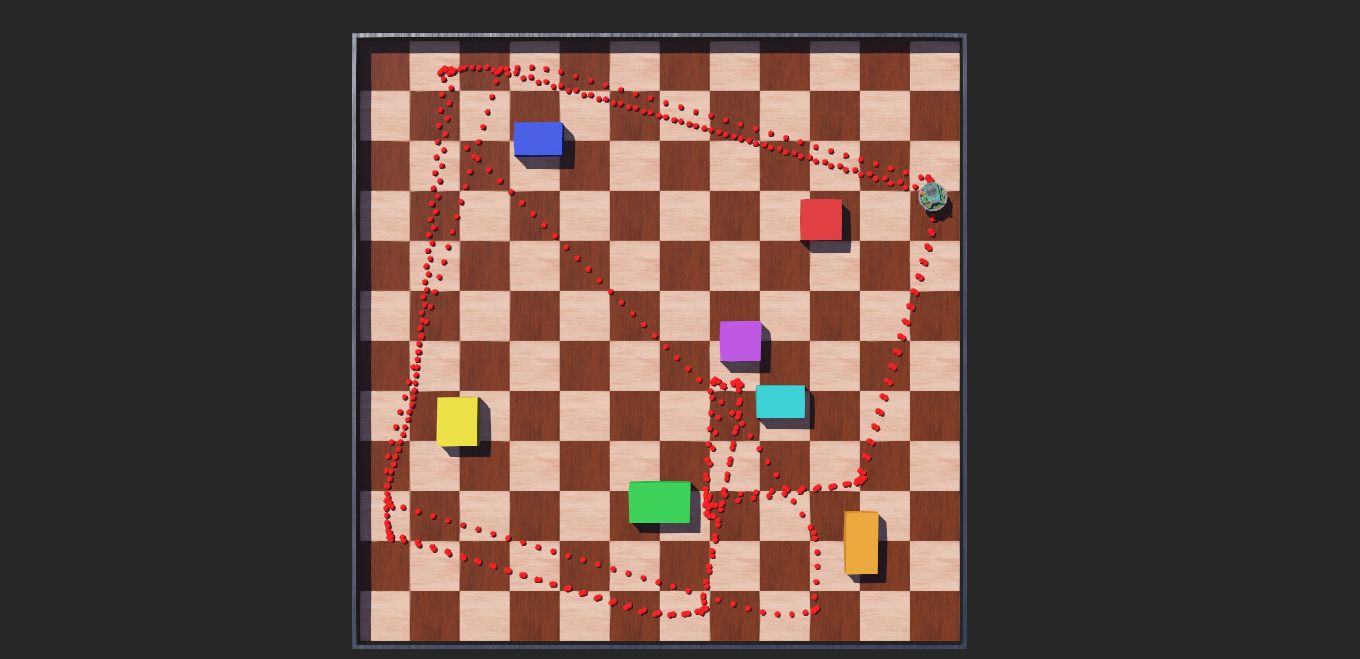
\includegraphics[width=0.85\textwidth]{Test Results/obstacle_avoidance_test_result5.png}
\caption{Test T5: Full arena endurance run (320 seconds) showing comprehensive coverage with zero collisions}
\label{fig:t5}
\end{figure}

\begin{figure}[H]
\centering
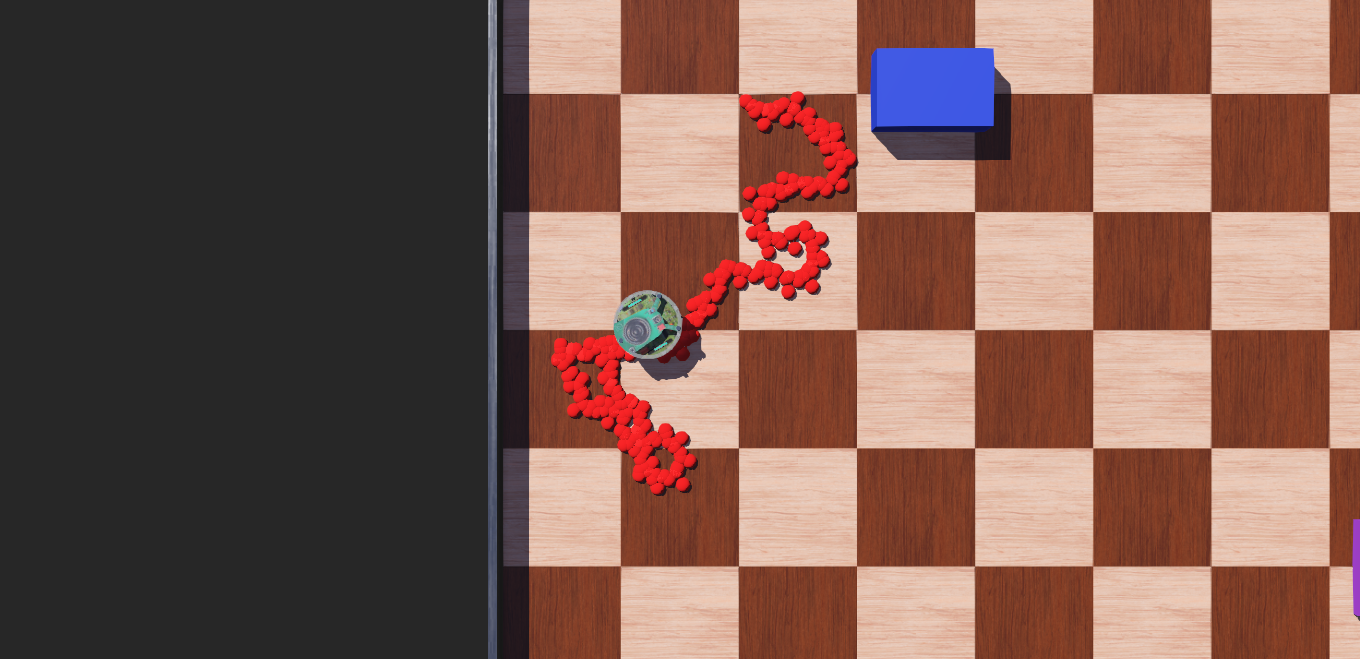
\includegraphics[width=0.45\textwidth]{Test Results/obstacle_avoidance_test_result6-rate-50.png}
\hfill
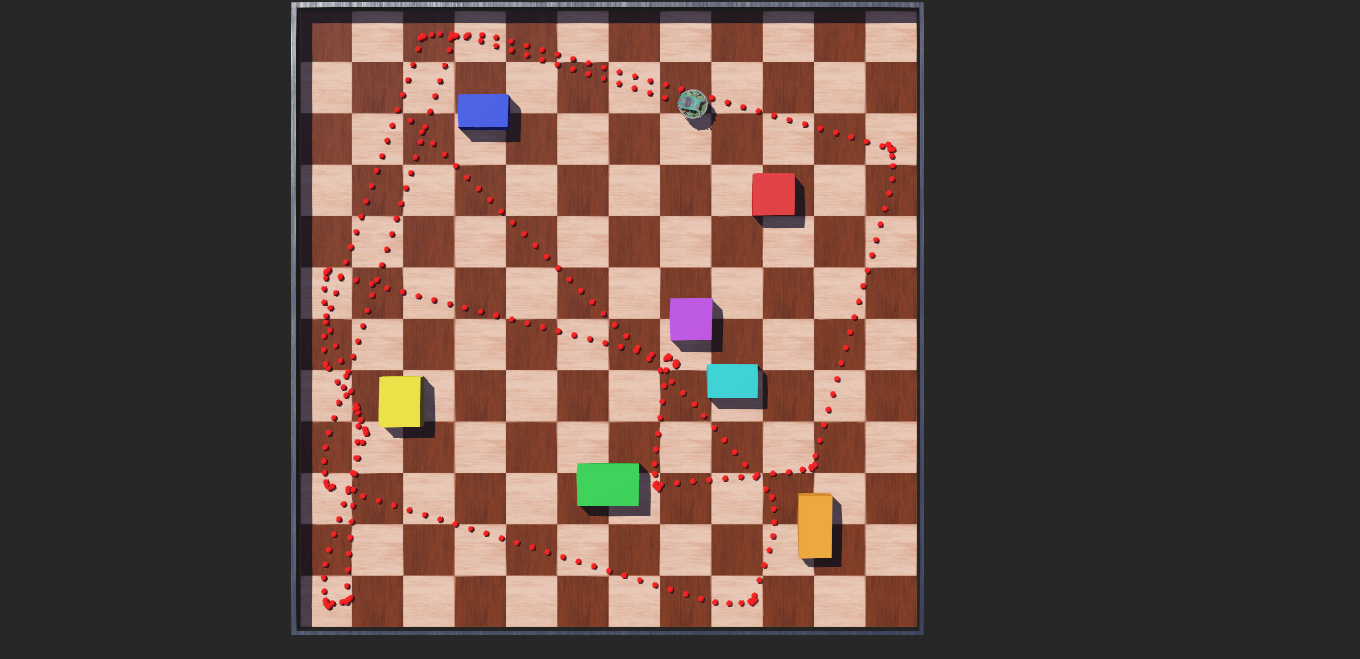
\includegraphics[width=0.45\textwidth]{Test Results/obstacle_avoidance_test_result6-rate-120.png}
\caption{Test T6: Threshold 50 (left) showing dysfunctional chaotic motion vs Threshold 120 (right) showing smooth paths}
\label{fig:t6}
\end{figure}

\begin{figure}[H]
\centering
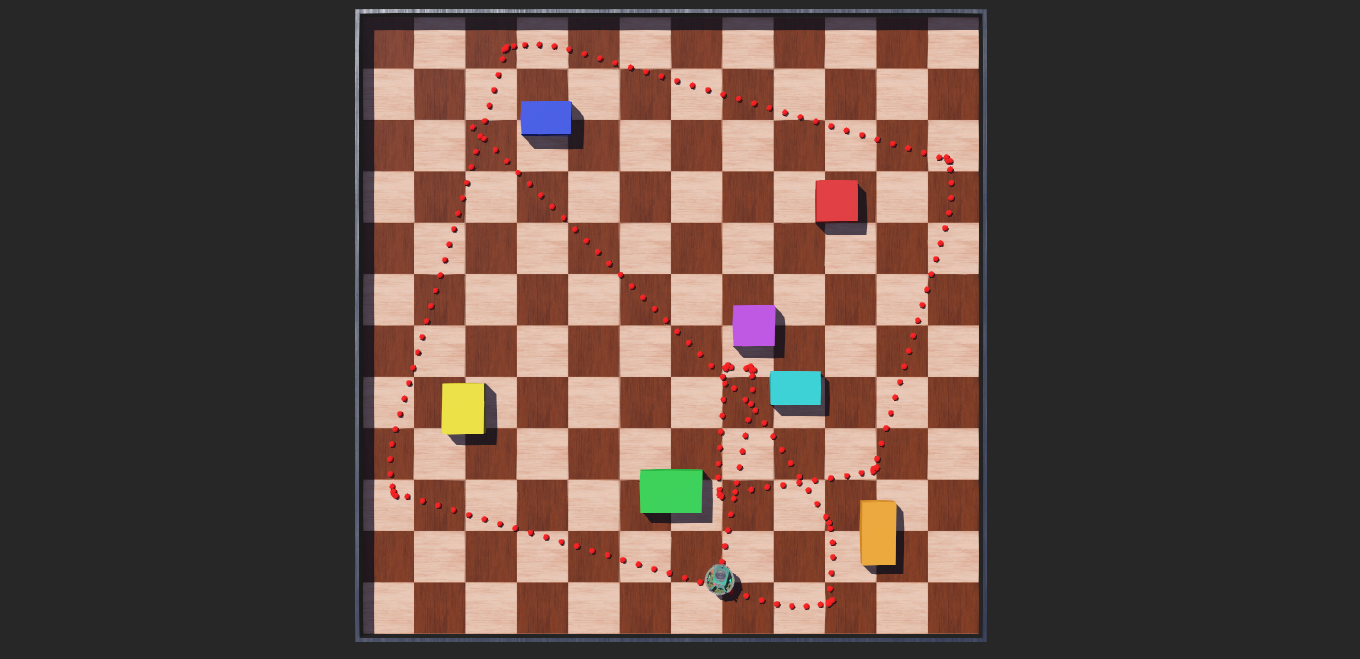
\includegraphics[width=0.85\textwidth]{Test Results/obstacle_avoidance_test_result2.png}
\caption{Test T2: Navigation through seven obstacles showing smooth curved avoidance paths}
\label{fig:t2}
\end{figure}

\subsection{Evaluation}

The project successfully met its stated criterion of one hundred percent collision avoidance across all test scenarios, including the most challenging corner trap and endurance tests. The proportional control approach proved highly effective, resolving 99.96\% of obstacle encounters without requiring the escape mechanism, which demonstrates that the Braitenberg-inspired graded response is sufficient for the vast majority of real-world navigation situations in this environment. The threshold sensitivity analysis provided the most significant engineering insight: the sensor noise floor of 60--76 units creates a hard lower bound on the detection threshold, and any setting below this floor renders the entire system non-functional regardless of all other parameter choices. This finding highlights the importance of empirical sensor characterisation before parameter tuning, as theoretical noise-free analysis would not reveal this constraint. The primary limitation is that the system operates only with static obstacles and has no mechanism to predict or react to moving objects, which would require velocity estimation and trajectory prediction. A secondary limitation is that without any form of path memory or coverage planning, the robot may revisit certain areas repeatedly while leaving others unexplored, though the endurance test trail shows that random exploration does eventually achieve good coverage over time. The infrared sensor detection range of approximately 8 centimetres limits how far ahead the robot can plan avoidance manoeuvres, meaning it must sometimes make sharp corrections for obstacles that appear suddenly at close range. Despite these limitations, the system demonstrates that reactive control with proportional response is a viable and effective approach for autonomous obstacle avoidance in structured environments.

% ══════════════════════════════════════════════════════════════════════════════
%  SECTION 5 - CONCLUSION
% ══════════════════════════════════════════════════════════════════════════════
\section{Conclusion}

\textbf{Conclusion.} This project successfully achieved its stated goal of one hundred percent collision avoidance across all six structured test scenarios, including open arena navigation, obstacle-dense environments, corner traps, narrow passages, full-arena endurance runs, and threshold sensitivity analysis. The system sustained over 320 seconds of continuous autonomous operation in a cluttered environment containing seven static obstacles, demonstrating robust long-duration reliability with only two escape manoeuvre activations during the entire endurance test. The reactive AI approach, inspired directly by Braitenberg's Vehicle 2a sensor-motor mapping, proved that complex and smooth navigation behaviour can emerge from simple proportional control rules without requiring path planning, mapping algorithms, or machine learning. However, the project has notable shortcomings: it was tested exclusively with static obstacles and would likely fail against moving objects without additional velocity-estimation logic; the robot has no coverage strategy and may leave areas unexplored while repeatedly visiting others; and the system requires manual threshold calibration that depends on the specific sensor hardware's noise characteristics. The corner trap scenario revealed that while the escape mechanism works, it sometimes requires multiple attempts (three in the worst case) to free the robot, suggesting that a more intelligent directional escape strategy could improve efficiency. The threshold sensitivity analysis exposed the most critical engineering insight: a single poorly chosen parameter (threshold below the 76-unit noise floor) renders an otherwise well-designed system completely non-functional, producing constant erratic false-positive detections. For someone attempting a similar project, the single most important actionable recommendation is to begin by characterising your sensor's ambient noise floor through a stationary measurement before choosing any detection threshold, because this one parameter determines whether the entire system functions or fails, regardless of how sophisticated the remaining control logic may be. Future work should explore dynamic obstacle handling through velocity estimation, systematic coverage algorithms using odometry, and adaptive threshold calibration that automatically adjusts to sensor drift over time.

% ══════════════════════════════════════════════════════════════════════════════
%  REFERENCES
% ══════════════════════════════════════════════════════════════════════════════
\vspace{0.5cm}

\begin{thebibliography}{9}

\bibitem{braitenberg1984}
Braitenberg, V. (\textbf{1984}). \textit{Vehicles: Experiments in Synthetic Psychology}. MIT Press. Available at: \url{https://mitpress.mit.edu/9780262521123/vehicles/}

\bibitem{brooks1986}
Brooks, R.A. (\textbf{1986}). A robust layered control system for a mobile robot. \textit{IEEE Journal on Robotics and Automation}, 2(1), pp. 14-23. Available at: \url{https://ieeexplore.ieee.org/document/1087032/}

\bibitem{mondada2009}
Mondada, F., Bonani, M., Raemy, X., Pugh, J., Cianci, C., Klaptocz, A., Magnenat, S., Zufferey, J.-C., Floreano, D., and Martinoli, A. (\textbf{2009}). The e-puck, a robot designed for education in engineering. \textit{Proceedings of the 9th Conference on Autonomous Robot Systems and Competitions}, 1(1), pp. 59-65. Available at: \url{https://infoscience.epfl.ch/record/135236}

\bibitem{webots2023}
Cyberbotics Ltd. (\textbf{2023}). \textit{Webots User Guide}. Available at: \url{https://cyberbotics.com/doc/guide/index}

\bibitem{webotsepuck2023}
Webots Reference Manual (\textbf{2023}). \textit{E-puck Documentation}. Cyberbotics Ltd. Available at: \url{https://cyberbotics.com/doc/guide/epuck}

\end{thebibliography}

\end{document}
